
\section{5. Architecture Integration}

\subsection{5.1 Model Support}

\begin{table}[H]
\centering
\begin{tabular}{lllll}
\toprule
\textbf{Architecture} & \textbf{Attention} & \textbf{RoPE?} & \textbf{GQA?} & \textbf{Verified} \\
\midrule
DistilBERT & Flat & No & No &  \\
RoBERTa & Nested & No & No &  \\
GPT-2 & Causal & No & No &  \\
Qwen3.5 & Causal + RoPE & Yes & Yes & {{Q\_VERIFIED}} \\
\bottomrule
\end{tabular}
\end{table}

\subsection{5.2 Weight Transfer}

\subsubsection{5.2.1 DistilBERT (Flat)}

Direct copy of \texttt{q\\_lin, k\\_lin, v\\_lin, out\\_lin}. \texttt{is\\_nested\\_encoder = False}.

\subsubsection{5.2.2 RoBERTa (Nested)}

Extract from inner \texttt{self}. \texttt{is\\_nested\\_encoder = True}; skip own \texttt{out\\_proj}.

\subsubsection{5.2.3 GPT-2 (Causal)}

Split fused \texttt{c\\_attn}:

\begin{lstlisting}
w = src.c_attn.weight.t()  # Conv1D transpose
q_w, k_w, v_w = w.chunk(3, dim=0)
\end{lstlisting}

\subsubsection{5.2.4 Qwen3.5 (GQA + RoPE)}

Direct copy with \texttt{repeat\\_kv} at runtime.

\subsection{5.3 Handling Nested Encoders}

For RoBERTa/BERT, \texttt{is\\_nested\\_encoder = True}:
\begin{itemize}
\item No \texttt{out\\_proj} applied inside NHA.
\end{itemize}
\begin{itemize}
\item Outer \texttt{attention.output.dense} applies output projection.
\end{itemize}

\subsection{5.4 Causality}

\begin{itemize}
\item \textbf{Local stream:} Band mask with $j \le i$.
\end{itemize}
\begin{itemize}
\item \textbf{Global stream:} Chunked prefix scan.
\end{itemize}

\subsection{5.5 RoPE Integration}

RoPE applied to Q, K \textbf{before} both streams:

\begin{lstlisting}
Q, K = apply_rotary_pos_emb(Q, K, cos, sin, position_ids)
\end{lstlisting}

\subsection{5.6 Padding Handling}

Both streams handle padding:
\begin{itemize}
\item \textbf{Local:} Mask invalid keys.
\end{itemize}
\begin{itemize}
\item \textbf{Global:} Zero out invalid K, V before prefix scan.
\end{itemize}

\subsection{5.7 Injection Algorithm}

\textbf{Algorithm 2:} Inject NHA into a full model
\begin{lstlisting}
Input:  model M, config c
Output: M with NHA attention

1:  for   in transformer_layers(M) do
2:      src $\leftarrow$ extract_attention( )
3:      if src is None: continue
4:      new $\leftarrow$ NativeHybridAttention(config=c, pretrained_attn=src)
5:      replace_attention( , new)
6: end for
\end{lstlisting}

\subsection{5.8 Failure Handling}

\texttt{inject\\_nha} returns \texttt{None} on failure:

\begin{lstlisting}
try:
    new_attn = NativeHybridAttention(...)
except Exception as e:
    logger.error("NHA construction failed: %s", e)
    return None
\end{lstlisting}

\subsection{5.9 Parameter Count}

\begin{table}[H]
\centering
\begin{tabular}{ll}
\toprule
\textbf{Projection} & \textbf{Params} \\
\midrule
$W_Q$ & $d H d_h$ \\
$W_K$ & $d H_{kv} d_h$ \\
$W_V$ & $d H_{kv} d_h$ \\
$W_O$ & $H d_h d$ \\
Gate & $d + 1$ \\
RFF buffer & $d_h m$ (not trainable) \\
\bottomrule
\end{tabular}
\end{table}

\subsection{5.10 Registry}

\begin{lstlisting}
@ATTENTION_REGISTRY.register("nha")
@ATTENTION_REGISTRY.register("nha_attention")
class NativeHybridAttention(BaseAttention): ...
\end{lstlisting}

\subsection{5.11 Failure Modes}


\begin{figure}[H]
\centering
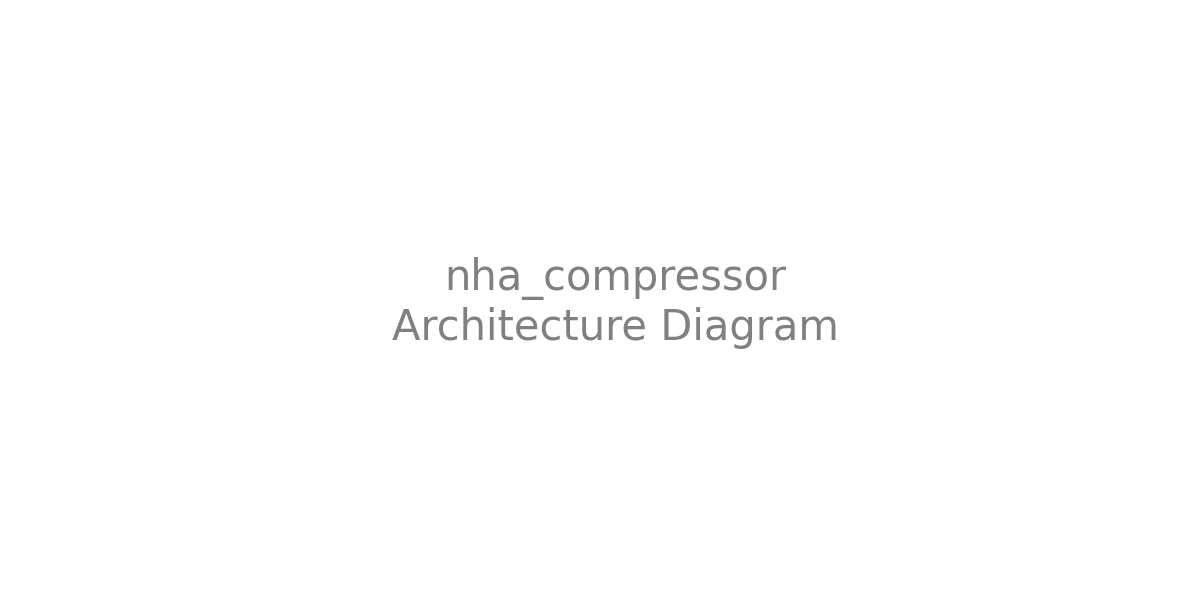
\includegraphics[width=\linewidth]{figures/nha_compressor_architecture.png}
\caption{Architectural overview of nha.}
\label{fig:arch_nha}
\end{figure}
